% ============================================================
%  Programación Científica 2026-1 — UNAL
%  Módulo: Integración Numérica
%  Clase única (90 min)
% ============================================================
\documentclass[aspectratio=169,10pt]{beamer}

% ---------- fuente sans-serif limpia ----------
\usepackage[T1]{fontenc}
\usepackage{helvet}
\renewcommand{\familydefault}{\sfdefault}

% ---------- paquetes ----------
\usepackage{amsmath,amssymb,bm}
\usepackage{tikz}
\usetikzlibrary{positioning,arrows.meta,calc,matrix,decorations.pathreplacing,shapes.geometric}
\usepackage{tcolorbox}
\tcbuselibrary{skins,breakable}
\usepackage{listings}
\usepackage{booktabs}
\usepackage{colortbl}
\usepackage{graphicx}
\usepackage{xcolor}

% ============================================================
%  PALETA DE COLORES
% ============================================================
\definecolor{darkbg}{HTML}{1C1C2E}
\definecolor{lightbg}{HTML}{F7F7F9}
\definecolor{accent}{HTML}{6C63FF}
\definecolor{accentteal}{HTML}{1DB89A}
\definecolor{accentamber}{HTML}{F4A623}
\definecolor{accentcoral}{HTML}{E05A4E}
\definecolor{textdark}{HTML}{1C1C2E}
\definecolor{textlight}{HTML}{F7F7F9}
\definecolor{textgray}{HTML}{6B6B80}
\definecolor{codefg}{HTML}{E8E8F0}
\definecolor{codebg}{HTML}{272740}

% ============================================================
%  TEMA BEAMER
% ============================================================
\setbeamertemplate{navigation symbols}{}
\setbeamertemplate{footline}{
	\begin{beamercolorbox}[wd=\paperwidth,ht=2.2ex,dp=1.2ex,rightskip=4mm]{footline}
		\hfill\usebeamerfont{footline}%
		\textcolor{textgray}{\tiny Programación Científica 2026-1 \quad|\quad
			Integración Numérica \quad|\quad \insertframenumber/\inserttotalframenumber}%
		\hspace{2mm}
	\end{beamercolorbox}
}

\setbeamercolor{normal text}{fg=textdark,bg=lightbg}
\setbeamercolor{frametitle}{fg=textdark,bg=lightbg}
\setbeamertemplate{frametitle}{
	\vspace{4pt}
	\begin{beamercolorbox}[wd=\textwidth,leftskip=2mm]{frametitle}
		\usebeamerfont{frametitle}\insertframetitle
		\ifx\insertframesubtitle\empty\else
		\par\vspace{1pt}
		{\footnotesize\textcolor{textgray}\insertframesubtitle}
		\fi
	\end{beamercolorbox}
	\vspace{-2pt}
	{\color{accent}\rule{\textwidth}{0.6pt}}
	\vspace{2pt}
}
\setbeamerfont{frametitle}{size=\large,series=\bfseries}

% ============================================================
%  CAJAS DE CONTENIDO
% ============================================================
\newtcolorbox{defbox}[1]{
	enhanced, title=#1,
	colback=accent!8, colframe=accent, coltitle=white,
	fonttitle=\bfseries\small, boxrule=0.6pt,
	attach boxed title to top left={yshift=-2mm,xshift=4mm},
	boxed title style={colback=accent,boxrule=0pt},
	left=4pt,right=4pt,top=6pt,bottom=4pt
}

\newtcolorbox{resultbox}[1]{
	enhanced, title=#1,
	colback=accentteal!8, colframe=accentteal, coltitle=white,
	fonttitle=\bfseries\small, boxrule=0.6pt,
	attach boxed title to top left={yshift=-2mm,xshift=4mm},
	boxed title style={colback=accentteal,boxrule=0pt},
	left=4pt,right=4pt,top=6pt,bottom=4pt
}

\newtcolorbox{obsbox}[1]{
	enhanced, title=#1,
	colback=accentamber!10, colframe=accentamber, coltitle=white,
	fonttitle=\bfseries\small, boxrule=0.6pt,
	attach boxed title to top left={yshift=-2mm,xshift=4mm},
	boxed title style={colback=accentamber,boxrule=0pt},
	left=4pt,right=4pt,top=6pt,bottom=4pt
}

\newtcolorbox{taskbox}[1]{
	enhanced, title=#1,
	colback=accentcoral!8, colframe=accentcoral, coltitle=white,
	fonttitle=\bfseries\small, boxrule=0.6pt,
	attach boxed title to top left={yshift=-2mm,xshift=4mm},
	boxed title style={colback=accentcoral,boxrule=0pt},
	left=4pt,right=4pt,top=6pt,bottom=4pt
}

% ============================================================
%  CÓDIGO
% ============================================================
\lstset{
	language=Python,
	basicstyle=\ttfamily\scriptsize\color{codefg},
	backgroundcolor=\color{codebg},
	keywordstyle=\color{accent!80!white}\bfseries,
	stringstyle=\color{accentteal},
	commentstyle=\color{textgray}\itshape,
	numbers=none,
	frame=none,
	breaklines=true,
	xleftmargin=4pt, xrightmargin=4pt,
	aboveskip=4pt, belowskip=4pt,
	showstringspaces=false,
	morekeywords={jnp,jax,np,scipy,integrate,trapz,simpson}
}

% ============================================================
%  SLIDE OSCURO
% ============================================================
\newcommand{\darkslide}[1]{
	{
		\setbeamercolor{background canvas}{bg=darkbg}
		\setbeamertemplate{footline}{}
		#1
	}
}

% ============================================================
%  MACROS MATEMÁTICOS
% ============================================================
\newcommand{\R}{\mathbb{R}}
\newcommand{\C}{\mathbb{C}}
\newcommand{\norm}[1]{\left\|#1\right\|}
\newcommand{\adj}{{}^{H}}

% ============================================================
%  PORTADA
% ============================================================
\title{\textbf{Integración Numérica}}
\subtitle{Módulo 4}
\author{Programación Científica 2026-1}
\institute{Universidad Nacional de Colombia}
\date{}

% ============================================================
\begin{document}
	% ============================================================
	
	% ---------- PORTADA ----------
	\darkslide{
		\begin{frame}[plain]
			\begin{tikzpicture}[remember picture, overlay]
				\fill[accent,opacity=0.15] (current page.north east) ++(-1,-1) circle (3.5cm);
				\fill[accentteal,opacity=0.10] (current page.south west) ++(2,2) circle (2.8cm);
				\fill[accentamber,opacity=0.08] (current page.south east) ++(-3,3) circle (1.8cm);
			\end{tikzpicture}
			\vspace{1.5cm}
			\begin{center}
				{\small\textcolor{accentteal}{\texttt{Programación Científica · UNAL · 2026-1}}}\\[10pt]
				{\LARGE\bfseries\textcolor{textlight}{Integración Numérica}}\\[6pt]
				{\large\textcolor{accent}{Módulo 4}}\\[18pt]
				{\small\textcolor{textgray}{Cuadratura · Regla del Trapecio · Regla de Simpson}}
			\end{center}
		\end{frame}
	}
	
	% ============================================================
	%  PARTE 1: MOTIVACIÓN
	% ============================================================
	\darkslide{
		\begin{frame}[plain]
			\begin{tikzpicture}[remember picture, overlay]
				\fill[accentteal,opacity=0.12] (current page.north west) ++(1,-1) circle (2.5cm);
				\fill[accent,opacity=0.10] (current page.south east) ++(-2,1.5) circle (2cm);
			\end{tikzpicture}
			\vspace{2.2cm}
			\begin{center}
				{\LARGE\bfseries\textcolor{textlight}{¿Cómo calculamos el área cuando no hay fórmula?}}
			\end{center}
		\end{frame}
	}
	
	% ----------
	\begin{frame}{El problema}
		\vspace{6pt}
		Queremos evaluar la integral definida:
		\[
		I = \int_{a}^{b} f(x) \, dx
		\]
		
		\vspace{4pt}
		Sabemos por el Teorema Fundamental del Cálculo que si $F'(x) = f(x)$, entonces $I = F(b) - F(a)$.
		
		\vspace{10pt}
		\begin{defbox}{El obstáculo}
			¿Qué pasa si $F(x)$ no se puede expresar con funciones elementales? \\
			¿O si \textbf{solo tenemos datos experimentales} medidos en puntos discretos $x_i$?
		\end{defbox}
		
		\vspace{8pt}
		\textcolor{textgray}{Necesitamos aproximar el valor de la integral sumando áreas geométricas.}
	\end{frame}
	
	% ----------
	\begin{frame}{Cuadratura Numérica}
		\vspace{6pt}
		La idea central de la integración numérica (o cuadratura) es aproximar la integral como una \textbf{suma ponderada} de evaluaciones de la función:
		\[
		\int_{a}^{b} f(x) \, dx \;\approx\; \sum_{i=0}^{n} w_i \, f(x_i)
		\]
		
		\vspace{8pt}
		\begin{itemize}\small
			\item $x_i$: Nodos o puntos de evaluación.
			\item $w_i$: Pesos asociados a cada nodo.
		\end{itemize}
		
		\vspace{6pt}
		\begin{obsbox}{Estrategia de Newton-Cotes}
			Dividimos el intervalo $[a,b]$ en $n$ subintervalos de ancho $h = \frac{b-a}{n}$. Luego, interpolamos $f(x)$ usando polinomios de grado bajo (líneas, parábolas) en cada subintervalo e integramos ese polinomio de forma exacta.
		\end{obsbox}
	\end{frame}
	
	% ============================================================
	%  PARTE 2: MÉTODOS CLÁSICOS
	% ============================================================
	\darkslide{
		\begin{frame}[plain]
			
\begin{tikzpicture}[remember picture, overlay]
				\fill[accent,opacity=0.12] (current page.north east) ++(-1.5,-1) circle (3cm);
				\fill[accentteal,opacity=0.08] (current page.south west) ++(1.5,1) circle (2.2cm);
			\end{tikzpicture}
			\vspace{2.2cm}
			\begin{center}
				{\LARGE\bfseries\textcolor{textlight}{Métodos de Newton-Cotes}}
			\end{center}
		\end{frame}
	}
	
	% ----------
	\begin{frame}{La Regla del Trapecio}
		\vspace{2pt}
		Aproximamos la función mediante una línea recta entre $f(x_i)$ y $f(x_{i+1})$. El área bajo esta línea es un trapecio.
		
		\vspace{6pt}
		\begin{columns}[T]
			\column{0.5\textwidth}
			Fórmula en un solo intervalo (tamaño $h$):
			\[
			\int_{x_i}^{x_{i+1}} f(x) \, dx \approx \frac{h}{2} \Big[ f(x_i) + f(x_{i+1}) \Big]
			\]
			
			\vspace{4pt}
			\textbf{Regla del Trapecio Compuesta} para $n$ intervalos:
			\[
			I \approx \frac{h}{2} \left[ f(x_0) + 2\sum_{i=1}^{n-1} f(x_i) + f(x_n) \right]
			\]
			
			\column{0.48\textwidth}
			\begin{center}
				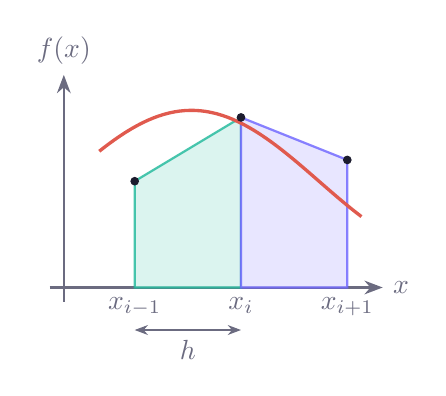
\begin{tikzpicture}[scale=0.9, >=Stealth]
					% axes
					\draw[->, textgray, thick] (-0.2, 0) -- (4.5, 0) node[right] {$x$};
					\draw[->, textgray, thick] (0, -0.2) -- (0, 3) node[above] {$f(x)$};
					% trapezoids
					\filldraw[fill=accentteal!20, draw=accentteal, thick, opacity=0.8] (1,0) -- (1,1.5) -- (2.5,2.4) -- (2.5,0) -- cycle;
					\filldraw[fill=accent!20, draw=accent, thick, opacity=0.8] (2.5,0) -- (2.5,2.4) -- (4,1.8) -- (4,0) -- cycle;
					% function curve
					\draw[very thick, accentcoral, domain=0.5:4.2, samples=50] plot (\x, {sin(\x*50)+1.5});
					% points and labels
					\filldraw[textdark] (1,1.5) circle (1.5pt);
					\filldraw[textdark] (2.5,2.4) circle (1.5pt);
					\filldraw[textdark] (4,1.8) circle (1.5pt);
					\node[below, textgray] at (1,0) {$x_{i-1}$};
					\node[below, textgray] at (2.5,0) {$x_i$};
					\node[below, textgray] at (4,0) {$x_{i+1}$};
					\draw[<->, textgray] (1,-0.6) -- node[below]{$h$} (2.5,-0.6);
				\end{tikzpicture}
			\end{center}
		\end{columns}
		
		\vspace{4pt}
		\textcolor{textgray}{\small \textit{El error global de la regla del trapecio escala como $\mathcal{O}(h^2)$.}}
	\end{frame}
	
	% ----------
	\begin{frame}{La Regla de Simpson}
		\vspace{6pt}
		En lugar de conectar los puntos con rectas, usamos grupos de \textbf{tres puntos} consecutivos $(x_{i-1}, x_i, x_{i+1})$ para ajustar una parábola (polinomio de grado 2).
		
		\vspace{10pt}
		\begin{resultbox}{Fórmula de Simpson $1/3$ (Compuesta)}
			Para aplicarla, el número de subintervalos $n$ \textbf{debe ser par}.
			\[
			I \approx \frac{h}{3} \left[ f(x_0) + 4\sum_{i \text{ impar}} f(x_i) + 2\sum_{i \text{ par}} f(x_i) + f(x_n) \right]
			\]
		\end{resultbox}
		
		\vspace{10pt}
		\textbf{Ventajas:}
		\begin{itemize}\small
			\item Gana mucha precisión con muy poco esfuerzo computacional extra.
			\item Su error global escala como $\mathcal{O}(h^4)$.
		\end{itemize}
	\end{frame}
	
	% ============================================================
	%  PARTE 3: IMPLEMENTACIÓN
	% ============================================================
	\darkslide{
		\begin{frame}[plain]
			\begin{tikzpicture}[remember picture, overlay]
				\fill[accentamber,opacity=0.10] (current page.north west) ++(2,-1.5) circle (3cm);
				\fill[accentcoral,opacity=0.10] (current page.south east) ++(-2,2) circle (2.5cm);
			\end{tikzpicture}
			\vspace{2.2cm}
			\begin{center}
				{\LARGE\bfseries\textcolor{textlight}{Integración en la práctica}}
			\end{center}
		\end{frame}
	}
	
	% ----------
	\begin{frame}[fragile]{Usando NumPy y SciPy}
		
		\vspace{4pt}
\begin{lstlisting}
import numpy as np
import scipy.integrate as integrate

# 1. Definir los nodos y la funcion
x = np.linspace(0, np.pi, 11)  # 10 paneles (11 puntos)
y = np.sin(x)

# 2. Regla del Trapecio (con NumPy)
I_trap = np.trapz(y, x)
print(f"Trapecio: {I_trap:.5f}")   # Salida: 1.98352

# 3. Regla de Simpson (con SciPy)
I_simp = integrate.simpson(y, x)
print(f"Simpson:  {I_simp:.5f}")   # Salida: 2.00011
\end{lstlisting}
		
	\end{frame}
	
	% ============================================================
	%  PARTE 1: CUADRATURA GAUSSIANA
	% ============================================================
	\darkslide{
		\begin{frame}[plain]
			\begin{tikzpicture}[remember picture, overlay]
				\fill[accentteal,opacity=0.12] (current page.north west) ++(1,-1) circle (2.5cm);
				\fill[accent,opacity=0.10] (current page.south east) ++(-2,1.5) circle (2cm);
			\end{tikzpicture}
			\vspace{2.2cm}
			\begin{center}
				{\LARGE\bfseries\textcolor{textlight}{Cuadratura Gaussiana}}
				\vspace{4pt}
				\par{\normalsize\textcolor{textgray}{¿Y si elegimos los puntos de forma inteligente?}}
			\end{center}
		\end{frame}
	}
	
	% ----------
	\begin{frame}{El límite de Newton-Cotes}
		\vspace{6pt}
		En Trapecio y Simpson, los puntos $x_i$ \textbf{están fijos y equidistantes}. Solo jugamos con los pesos $w_i$.
		
		\vspace{10pt}
		\begin{defbox}{La genialidad de Gauss}
			¿Qué pasa si tratamos tanto a los pesos $w_i$ como a las posiciones de los nodos $x_i$ como \textbf{incógnitas} y los optimizamos simultáneamente?
		\end{defbox}
		
		\vspace{8pt}
		\begin{itemize}\small
			\item Con $n$ puntos equidistantes, integramos polinomios de grado $n-1$ exactamente.
			\item Con $n$ puntos de Gauss, integramos polinomios de grado \textbf{$2n - 1$} exactamente. ¡El doble de precisión por el mismo costo computacional!
		\end{itemize}
	\end{frame}
	
	% ----------
	\begin{frame}{Regla de Gauss-Legendre (2 puntos)}
		\vspace{4pt}
		La fórmula estándar de cuadratura gaussiana está definida en el \textbf{intervalo canónico $[-1, 1]$}:
		\[
		\int_{-1}^{1} f(x) \, dx \approx \sum_{i=1}^{n} w_i f(x_i)
		\]
		
		\vspace{6pt}
		Para \textbf{$n=2$}, los parámetros óptimos (derivados matemáticamente) son:
		\begin{center}
			\begin{tabular}{ccc}
				\toprule
				\textbf{Punto} $i$ & \textbf{Nodo} $x_i$ & \textbf{Peso} $w_i$ \\
				\midrule
				1 & $-1/\sqrt{3} \approx -0.57735$ & $1$ \\
				2 & $1/\sqrt{3} \approx 0.57735$ & $1$ \\
				\bottomrule
			\end{tabular}
		\end{center}
		
		\begin{resultbox}{Fórmula de 2 puntos}
			\[
			\int_{-1}^{1} f(x) \, dx \approx f\left(-\frac{1}{\sqrt{3}}\right) + f\left(\frac{1}{\sqrt{3}}\right)
			\]
		\end{resultbox}
	\end{frame}
	
	
	% ============================================================
	%  PARTE 2: MONTE CARLO
	% ============================================================
	\darkslide{
		\begin{frame}[plain]
			\begin{tikzpicture}[remember picture, overlay]
				\fill[accentamber,opacity=0.12] (current page.north east) ++(-1.5,-1) circle (3cm);
				\fill[accentcoral,opacity=0.10] (current page.south west) ++(1.5,1.5) circle (2.5cm);
			\end{tikzpicture}
			\vspace{2.2cm}
			\begin{center}
				{\LARGE\bfseries\textcolor{textlight}{Integración de Monte Carlo}}
				\vspace{4pt}
				\par{\normalsize\textcolor{textgray}{El poder de la aleatoriedad en altas dimensiones}}
			\end{center}
		\end{frame}
	}
	
	% ----------
	\begin{frame}{La maldición de la dimensionalidad}
		\vspace{6pt}
		Gauss, Simpson y Trapecio son fantásticos en 1 dimensión. 
		Pero, ¿qué pasa si queremos integrar en 10 dimensiones?
		\[ \int \dots \int f(x_1, \dots, x_{10}) \, dx_1 \dots dx_{10} \]
		
		\vspace{6pt}
		Si usamos una malla de \textbf{apenas 10 puntos} por dimensión:
		\begin{itemize}
			\item $1D \rightarrow 10^1 = 10$ evaluaciones.
			\item $2D \rightarrow 10^2 = 100$ evaluaciones.
			\item $10D \rightarrow 10^{10} = 10.000.000.000$ evaluaciones.
		\end{itemize}
		
		\vspace{10pt}
		\begin{defbox}{El problema de los métodos de malla}
			El costo computacional crece exponencialmente con el número de dimensiones. A esto se le conoce como la \textbf{Maldición de la Dimensionalidad}.
		\end{defbox}
	\end{frame}
	
	% ----------
	\begin{frame}{La solución probabilística}
		\vspace{6pt}
		El método de \textbf{Monte Carlo} abandona las mallas estructuradas. En su lugar, lanza "dardos" al azar en el dominio de integración.
		
		\vspace{8pt}
		La fórmula básica del valor esperado en 1D es:
		\[ \int_{a}^{b} f(x) \, dx \approx \frac{b-a}{N} \sum_{i=1}^{N} f(x_i) \]
		Donde $x_1, x_2, \dots, x_N$ son números aleatorios generados de una distribución \textbf{uniforme} entre $a$ y $b$.
		
		\vspace{10pt}
		\begin{resultbox}{La magia de Monte Carlo}
			El error del método de Monte Carlo disminuye a una tasa de $\mathcal{O}(1/\sqrt{N})$, \textbf{independientemente del número de dimensiones}. En dimensiones altas, Monte Carlo no es solo una alternativa, ¡es la única opción!
		\end{resultbox}
	\end{frame}
	
	% ----------
	\begin{frame}[fragile]{Ejercicio Práctico: Estimando $\pi$ con Dardos}
		\vspace{2pt}
		\begin{columns}[T]
			\column{0.5\textwidth}
			Dado un cuadrado de lado 2 (área = 4) centrado en el origen. Dentro de él hay un círculo de radio 1 (área = $\pi$).
			
			Si lanzamos $N$ dardos aleatorios sobre el cuadrado, la probabilidad de caer dentro del círculo es:
			\[ P \approx \frac{\text{Área Círculo}}{\text{Área Cuadrado}} = \frac{\pi}{4} \]
			
			\vspace{4pt}
			\begin{obsbox}{Condición}
				Un dardo $(x, y)$ está dentro del círculo si:
				\[ x^2 + y^2 \le 1 \]
			\end{obsbox}
			
			\column{0.48\textwidth}
			\begin{taskbox}{Tu turno (En Python)}
				\begin{enumerate}\small
					\item Genere $N=10^6$ valores de $x$ aleatorios uniformes entre $[-1, 1]$.
					\item Genere $N=10^6$ valores de $y$ independientes entre $[-1, 1]$.
					\item Cuente cuántos puntos cumplen \texttt{x**2 + y**2 <= 1}.
					\item Multiplique esa fracción por el área del cuadrado (4).
					\item Imprima el error respecto a \texttt{np.pi}.
				\end{enumerate}
			\end{taskbox}
		\end{columns}
	\end{frame}
	
	
	% ============================================================
	%  SLIDE FINAL
	% ============================================================
	\darkslide{
		\begin{frame}[plain]
			\begin{tikzpicture}[remember picture, overlay]
				\fill[accent,opacity=0.15] (current page.north east) ++(-1,-1) circle (3.5cm);
				\fill[accentteal,opacity=0.10] (current page.south west) ++(2,2) circle (2.8cm);
			\end{tikzpicture}
			\begin{center}
					{\large\textcolor{textgray}{Recapitulando}}\\[14pt]
				{\large\textcolor{textlight}{\textbf{El Problema de Integrar}}}\\
				{\small\textcolor{textgray}{Aproximar el área sumando áreas geométricas conocidas}}\\[10pt]
				{\large\textcolor{textlight}{\textbf{Trapecio vs. Simpson}}}\\
				{\small\textcolor{textgray}{Interpolación lineal vs. cuadrática: $\mathcal{O}(h^2)$ vs $\mathcal{O}(h^4)$}}\\[10pt]
				{\large\textcolor{textlight}{\textbf{Cuadratura de Gauss}}}\\
				{\small\textcolor{textgray}{Puntos y pesos optimizados: el doble de precisión analítica}}\\[10pt]
				{\large\textcolor{textlight}{\textbf{Monte Carlo}}}\\
				{\small\textcolor{textgray}{Integración estocástica: invencible en dimensiones altas}}\\[50pt]
				{\small\textcolor{textgray}{\texttt{mbastidaso@unal.edu.co}}}
			\end{center}
		\end{frame}
	}

	
\end{document}